\subsubsection{Giao diện người dùng - Danh sách/Chi tiết công việc}

Khi truy cập vào trang danh sách công việc tuyển dụng, Front-end sẽ tự động fetch dữ liệu từ Backend thông qua một API tương tự như ở trang chủ: thực hiện phân trang để lấy lần lượt các công việc trong cơ sở dữ liệu dựa trên tham số \texttt{current} và \texttt{pageSize}.

\begin{figure}[H]
    \centering
    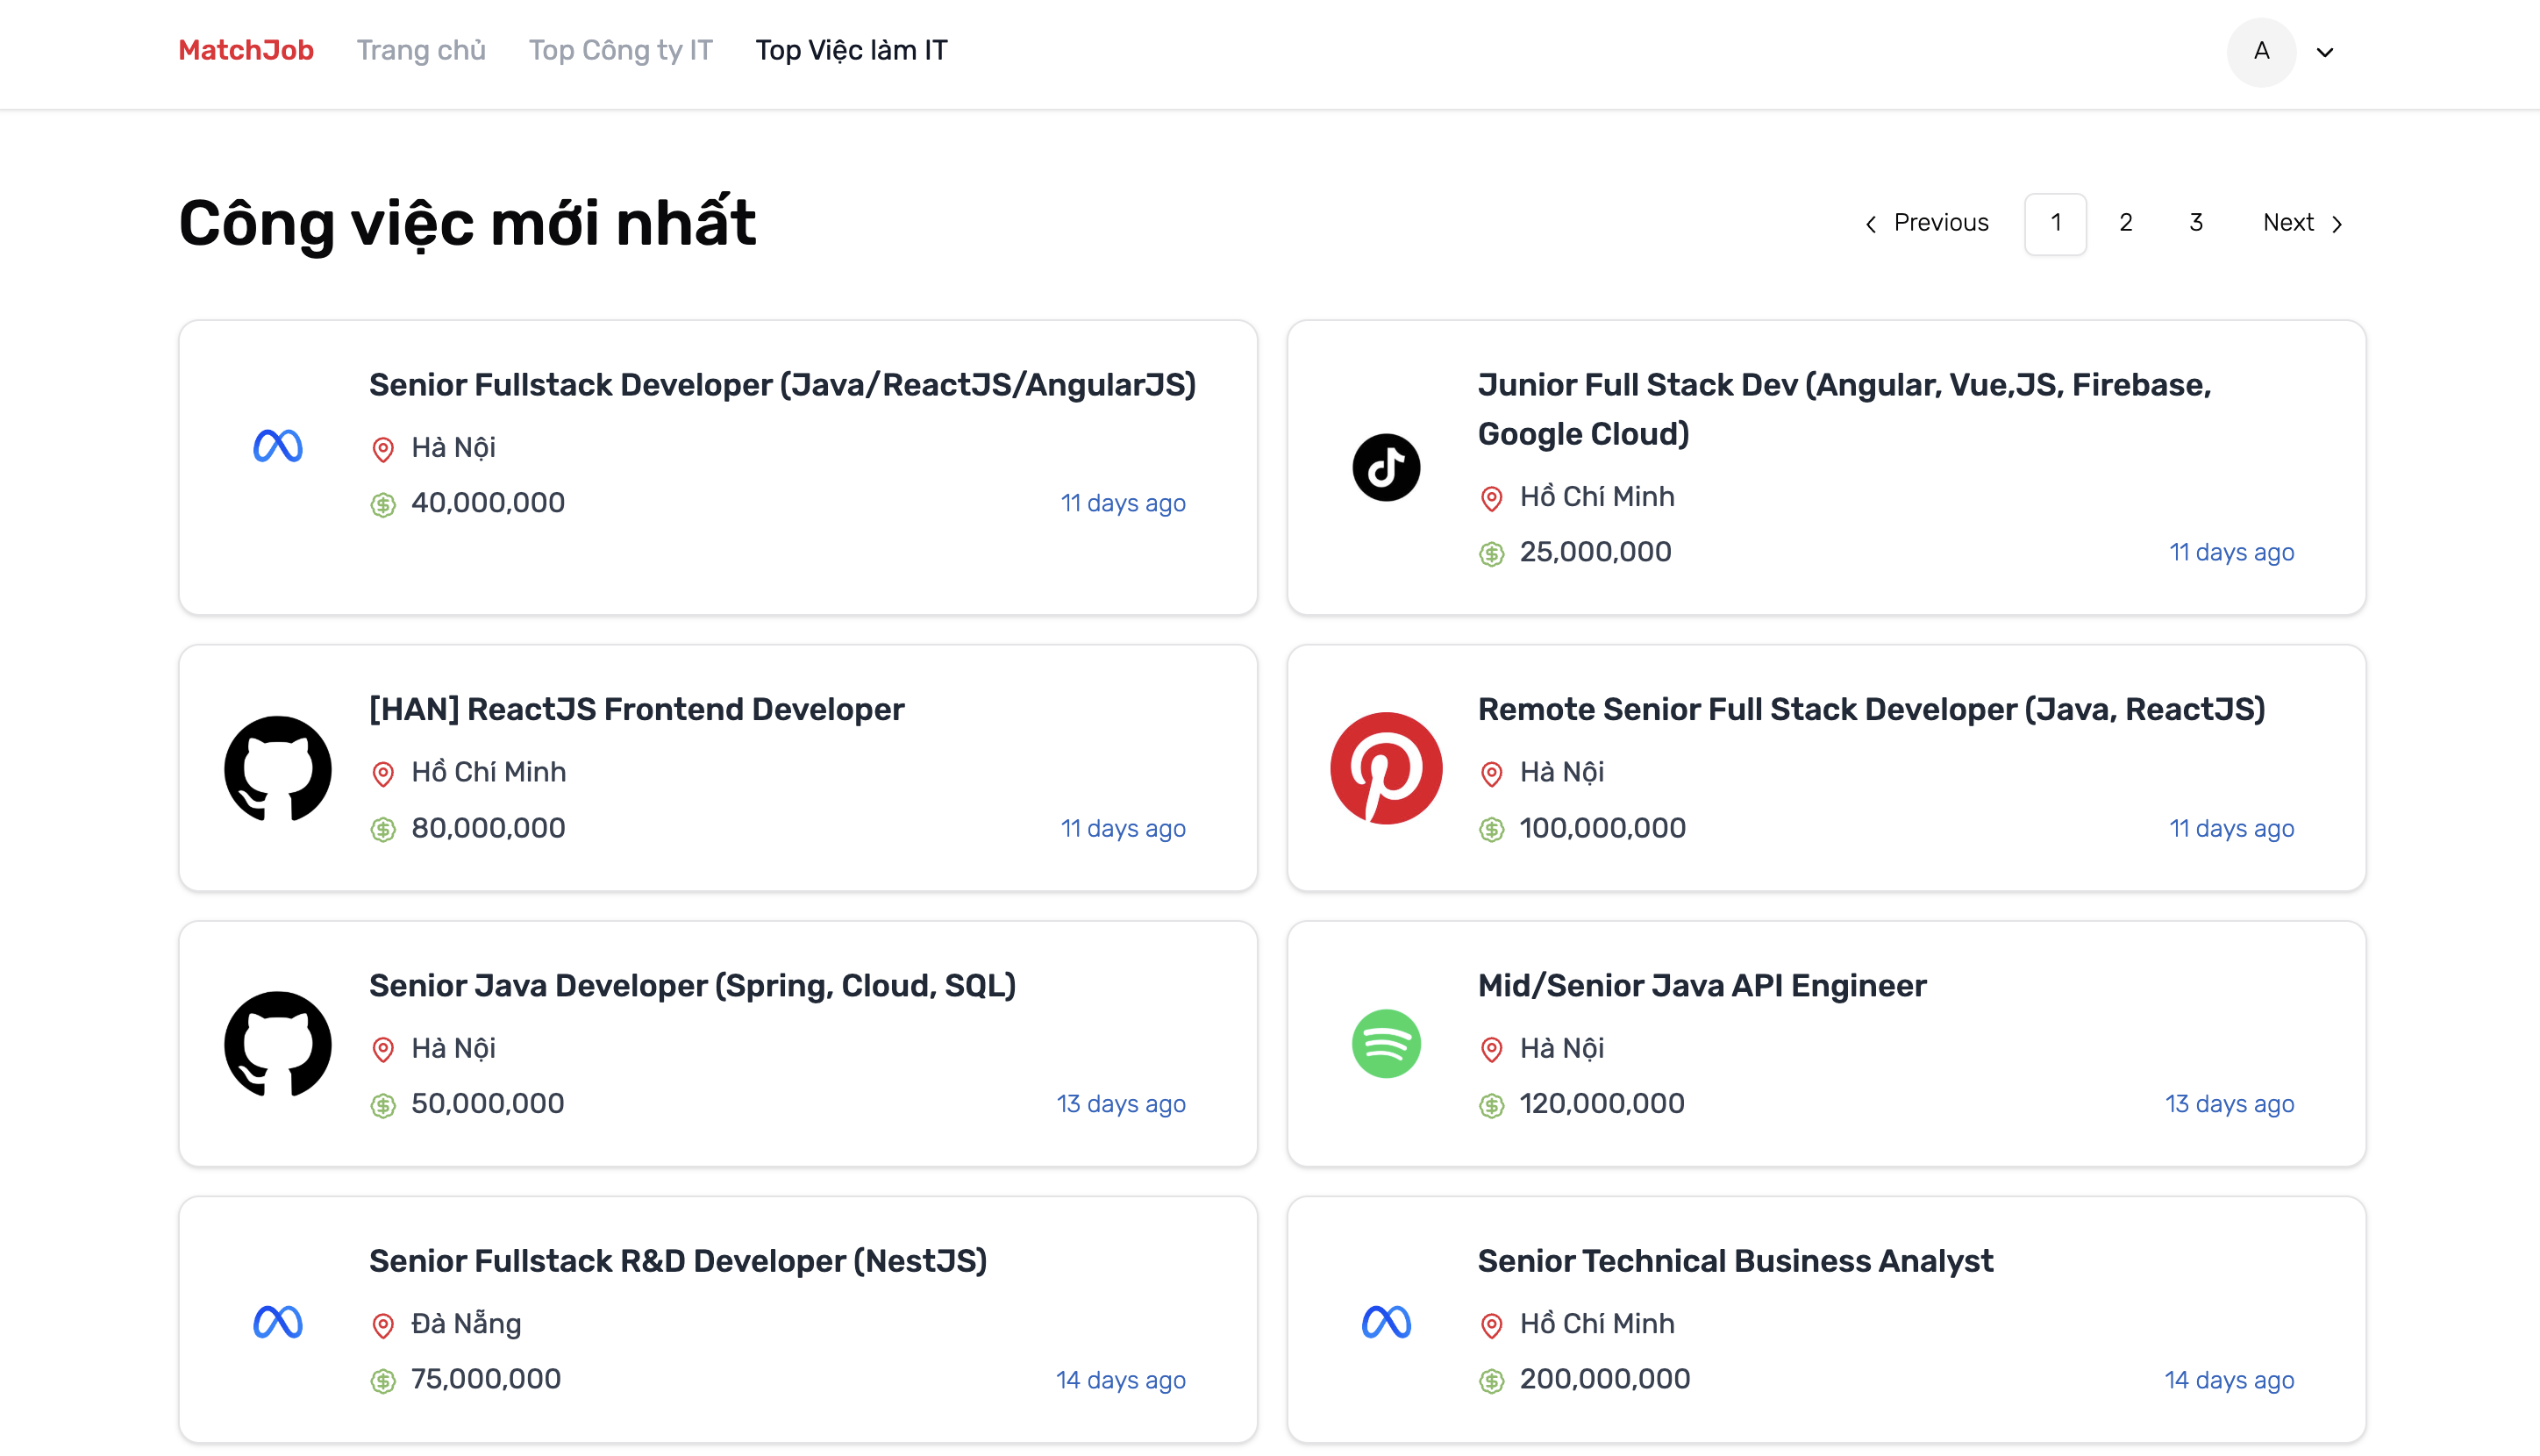
\includegraphics[width=\linewidth]{DBMS-Application/Images/list-job.png}
    \caption{Danh sách công việc đang được tuyển dụng}
\end{figure}

Và cũng như ở trang Danh sách công ty đã trình bày, người dùng cũng có thể chọn 1 công việc để xem chi tiết công việc đó:

\begin{figure}[H]
    \centering
    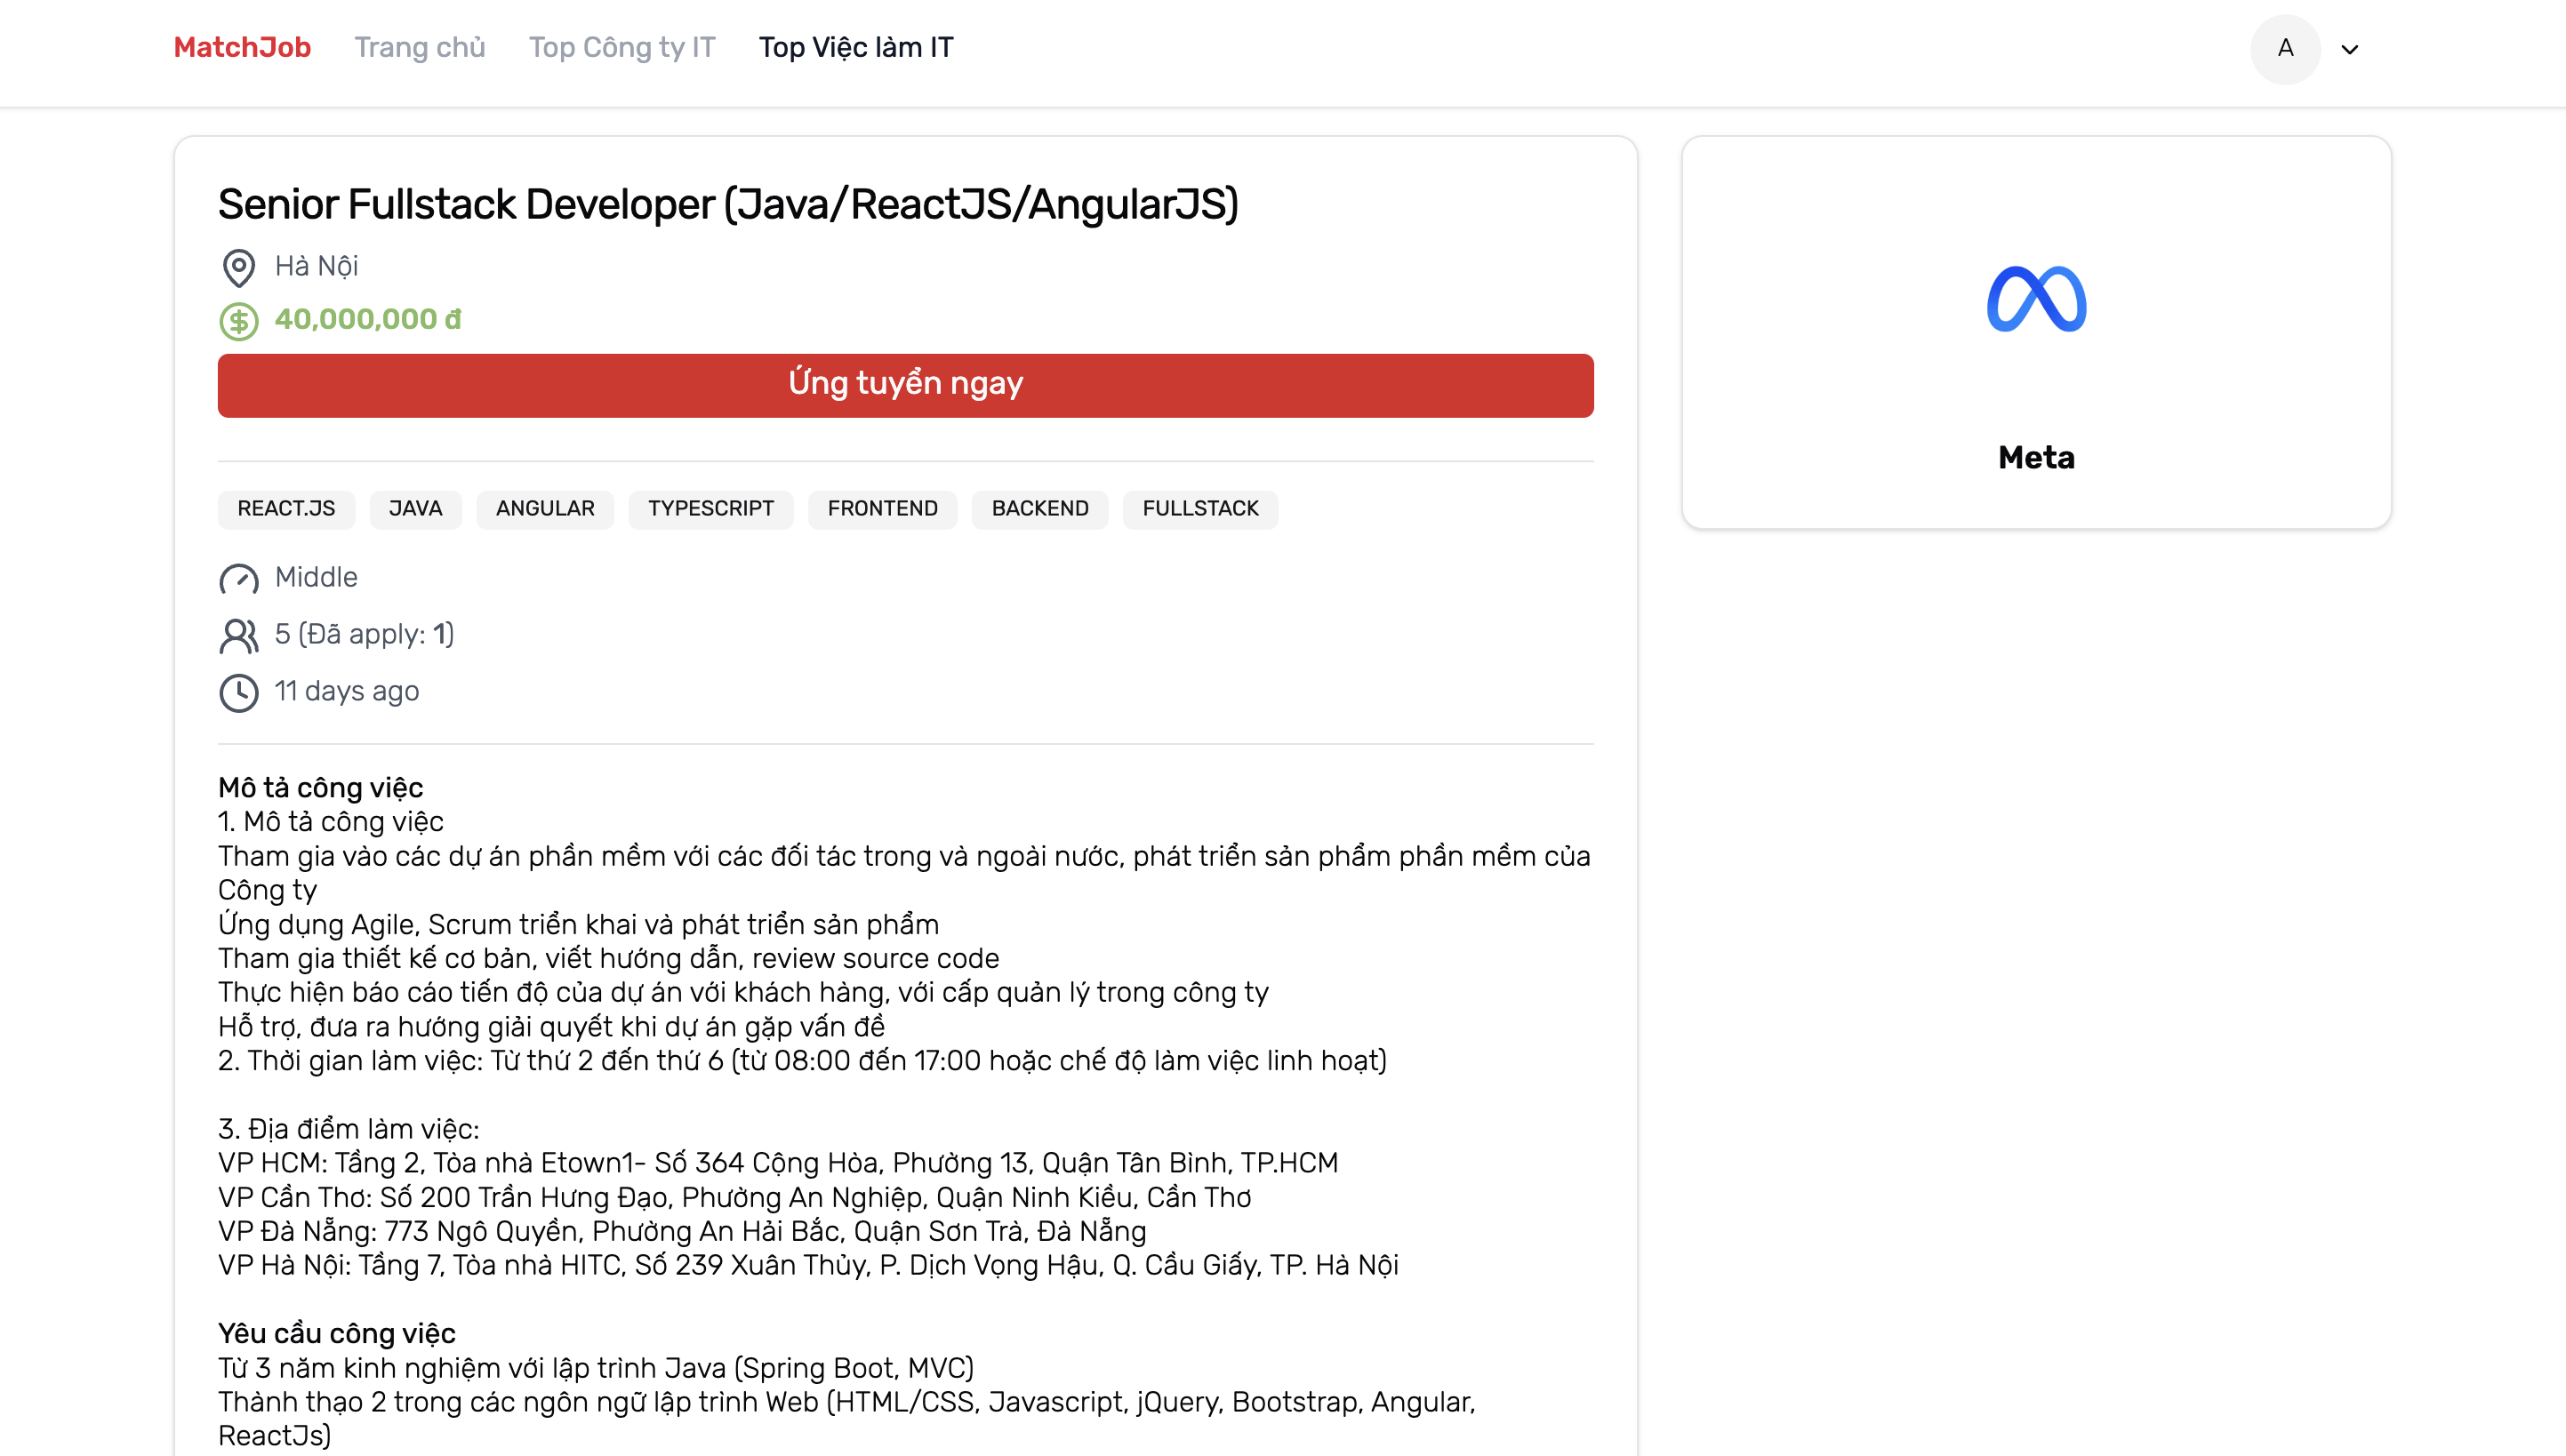
\includegraphics[width=\linewidth]{DBMS-Application/Images/job-detail.png}
    \caption{Danh sách công việc đang được tuyển dụng}
\end{figure}

Truy vấn sử dụng: \textbf{Query with single condition} - Sử dụng điều kiện \texttt{\_id} để tìm công việc duy nhất

\begin{lstlisting}
return await this.db
  .collection('jobs')
  .findOne({ _id: new ObjectId(id) });
\end{lstlisting}

Bên cạnh đó, hệ thống Front-end cũng tự động gửi yêu cầu thông qua API để lấy về số lượng hồ sơ đã nộp từ các ứng viên khác cho công việc hiện tại

\begin{figure}[H]
    \centering
    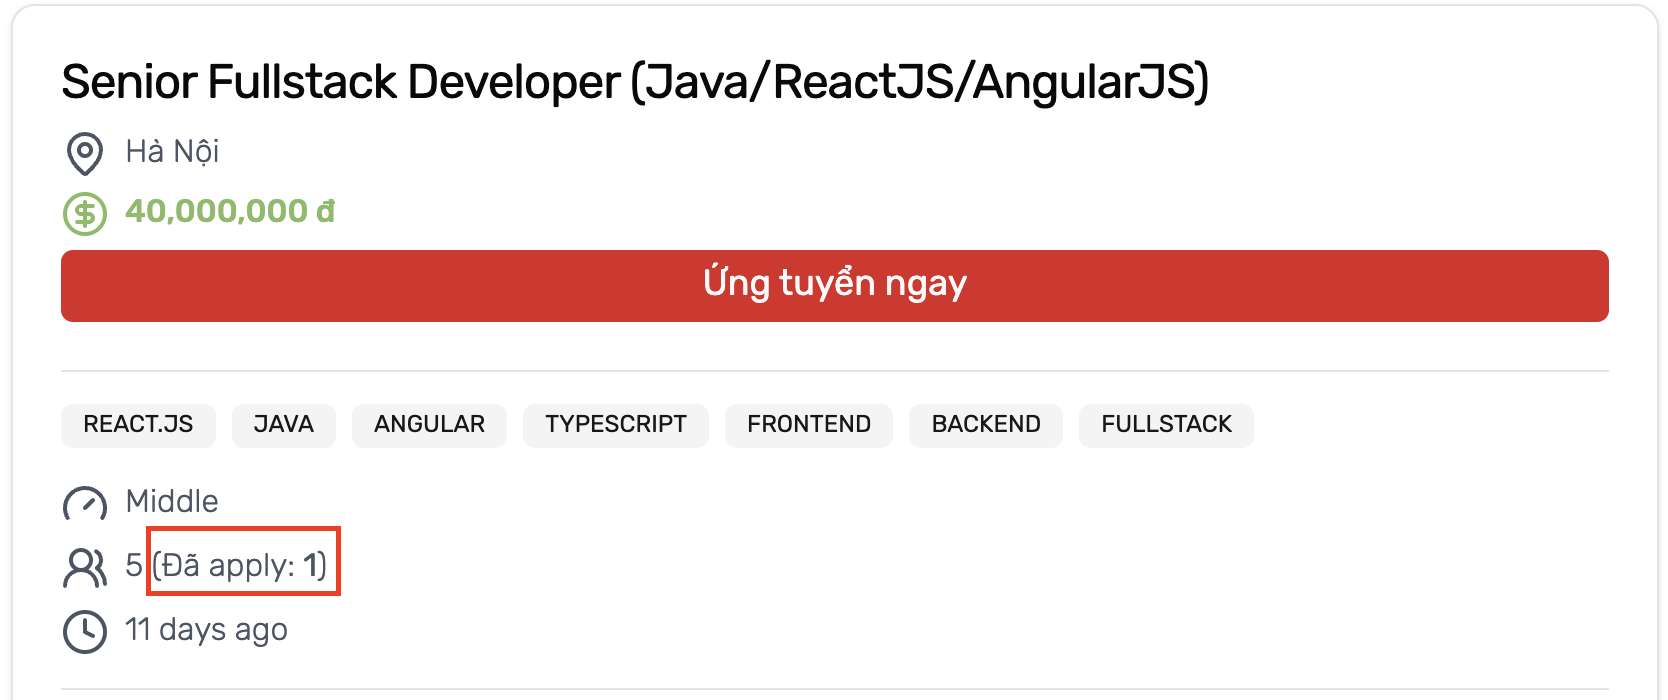
\includegraphics[width=.75\linewidth]{DBMS-Application/Images/number-resumes-apply.png}
    \caption{Số lượng hồ sơ đã được nộp cho công việc hiện tại}
\end{figure}

Truy vấn sử dụng:
\begin{itemize}
    \item \textbf{Query with single condition}: Sử dụng \texttt{\$match} để tìm một công việc cụ thể trong collection \textbf{jobs} dựa trên \texttt{\_id}
    
    \item \textbf{Query with join}: Thực hiện join thông qua \texttt{\$lookup} giữa collection \textbf{jobs} (\texttt{\_id}) và \textbf{resumes} (\texttt{jobId}) để lấy danh sách hồ sơ ứng tuyển của đến công việc đó

    \item \textbf{Query with aggregation functions}: Sử dụng \texttt{\$size} để tính tổng số lượng hồ sơ ứng tuyển của công việc
\end{itemize}

\begin{lstlisting}
const pipeline = [
  {
    $match: { _id: new ObjectId(id) }, // Tim job cu the thong qua _id
  },
  {
    $lookup: {
      from: 'resumes', // Join collection 'jobs' voi collection 'resumes'
      localField: '_id',
      foreignField: 'jobId',
      as: 'resumes',
    },
  },
  {
    $project: {
      _id: 1,
      totalResumes: { $size: '$resumes' }, // Dem so luong resumes da nop
    },
  },
];

const result = await this.db
  .collection('jobs')
  .aggregate(pipeline)
  .toArray();

return result[0];
\end{lstlisting}

Giải thích truy vấn:
\begin{itemize}
    \item \texttt{\$match}: Lọc công việc cụ thể từ collection \textbf{jobs} dựa trên \_id.
    \item \texttt{\$lookup}: Join với collection \textbf{resumes} để tìm các hồ sơ ứng tuyển có trường \texttt{jobId} trùng với \texttt{\_id} của công việc
    \item \texttt{\$project}: Trả về \texttt{\_id} của công việc và tổng số hồ sơ ứng tuyển (\texttt{totalResumes}) bằng cách sử dụng \texttt{\$size} để đếm số phần tử trong mảng resumes.
\end{itemize}

Cuối cùng, người dùng có thể upload (tạo) hồ sơ và apply cho công việc cụ thể:

\begin{figure}[H]
    \centering
    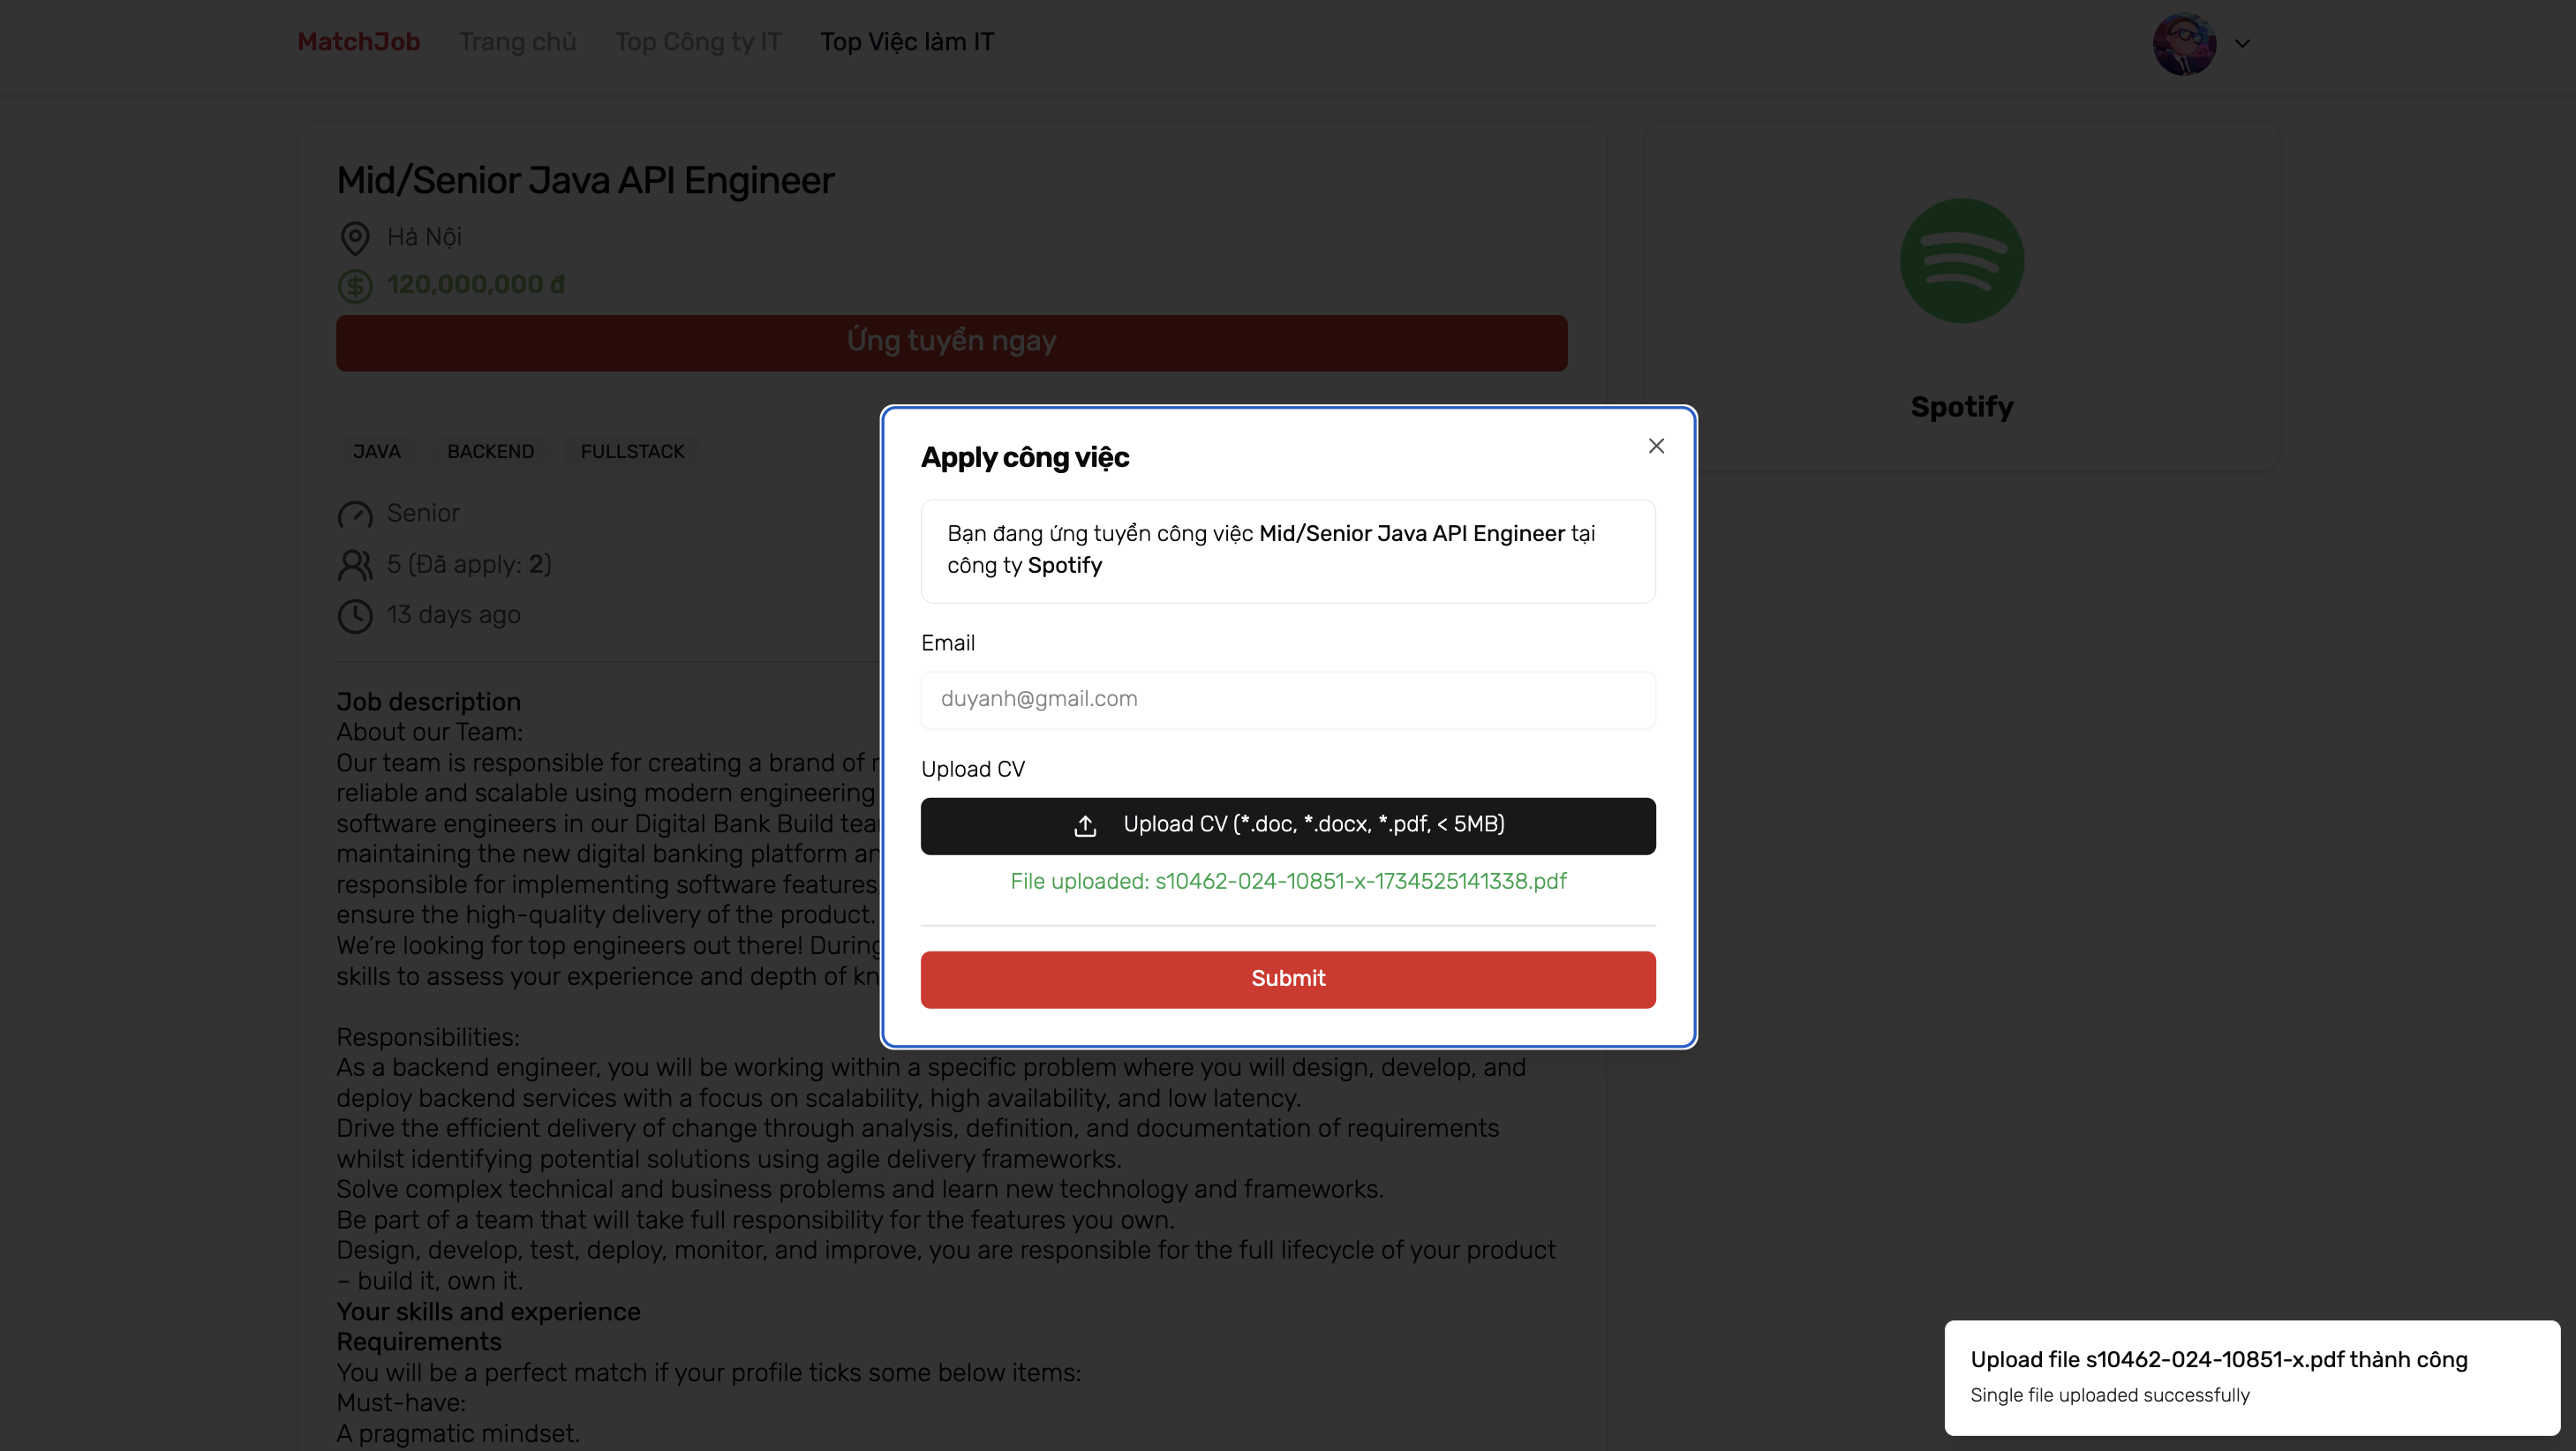
\includegraphics[width=\linewidth]{DBMS-Application/Images/modal-upload-cv.png}
    \caption{Số lượng hồ sơ đã được nộp cho công việc hiện tại}
\end{figure}

Truy vấn sử dụng: \textbf{Insert}

\begin{lstlisting}
const newResume = {
  url,
  companyId: new ObjectId(companyId),
  email,
  jobId: new ObjectId(jobId),
  userId: new ObjectId(_id),
  status: 'PENDING',
  createdAt: new Date(),
  updatedAt: new Date(),
};

const result = await this.db.collection('resumes').insertOne(newResume); // Them ho so ung tuyen moi vao database

return {
  _id: result.insertedId,
  createdAt: newResume.createdAt,
};

\end{lstlisting}
